\documentclass[12pt,oneside]{report}

% --- Packages ---
\usepackage[margin=1in]{geometry}
\usepackage{lmodern} % Latin Modern font
\usepackage[T1]{fontenc}
\usepackage{amsmath,amssymb}
\usepackage{graphicx}
\usepackage{booktabs,tabularx}
\usepackage{listings}
\usepackage{float}
\usepackage{algorithm}
\usepackage{algpseudocode}
\usepackage{fancyhdr}
\usepackage{titlesec}
\usepackage{caption}
\usepackage{microtype}
\usepackage{setspace}
\usepackage{color}
\usepackage[pdftex,bookmarksnumbered=true,colorlinks=true,linkcolor=black,citecolor=black,urlcolor=black]{hyperref}
\usepackage{bookmark}

\hypersetup{
    pdftitle={FinMetrics Suite: An AI-Powered Cross-Sectional Financial Analysis, Anomaly Detection, and Strategic Benchmarking System},
    pdfauthor={N Rohit Vedhanandh},
    pdfsubject={Corporate Internship},
    pdfkeywords={Financial Analysis, Anomaly Detection, Outlier Screening, Unsupervised Learning, K-Means Clustering, Isolation Forest, ERP Integration, TallySync, SWOT Grid, Strategic Benchmarking}
}

% --- TikZ Package & Libraries ---
\usepackage{tikz}
\usetikzlibrary{shapes.geometric, arrows, arrows.meta, positioning, calc}

% --- Custom Colors ---
\definecolor{codegreen}{rgb}{0,0.6,0}
\definecolor{codegray}{rgb}{0.5,0.5,0.5}
\definecolor{codeblue}{rgb}{0,0,0.8}
\definecolor{backgroundcolor}{rgb}{0.97,0.97,0.97}

% --- Code Listing Styling ---
\lstset{
    backgroundcolor=\color{backgroundcolor},
    commentstyle=\color{codegreen},
    keywordstyle=\color{codeblue},
    numberstyle=\tiny\color{codegray},
    stringstyle=\color{codegreen},
    basicstyle=\ttfamily\footnotesize,
    breakatwhitespace=false,
    breaklines=true,
    captionpos=b,
    keepspaces=true,
    numbers=left,
    numbersep=5pt,
    showspaces=false,
    showstringspaces=false,
    showtabs=false,
    tabsize=2
}

% --- Layout Configurations ---
\onehalfspacing
\pagestyle{fancy}
\fancyhf{}
\definecolor{charcoal}{rgb}{0.2,0.2,0.2}
\definecolor{headergray}{rgb}{0.7,0.7,0.7}
\definecolor{commentgray}{rgb}{0.5,0.5,0.5}
\fancyhead[L]{\textcolor{charcoal}{\small\nouppercase{\leftmark}}}
\fancyhead[R]{\textcolor{charcoal}{\small\thepage}}
\renewcommand{\headrule}{\hbox to\headwidth{\color{headergray}\leaders\hrule height 0.4pt\hfill}}
\renewcommand{\chaptermark}[1]{\markboth{#1}{}}
\setlength{\headheight}{25pt}
\addtolength{\topmargin}{-13pt}

% --- Algorithmic Styling Refinements ---
\renewcommand{\algorithmiccomment}[1]{\hfill\textcolor{commentgray}{\ensuremath{\triangleright}\ \textit{#1}}}

% --- Chapter Title Spacing Optimization (Reducing Top Whitespace) ---
\titleformat{\chapter}[display]
  {\normalfont\huge\bfseries}{\chaptername\ \thechapter}{10pt}{\Huge}
\titlespacing*{\chapter}{0pt}{-25pt}{20pt}

% --- Paragraph Spacing ---
\setlength{\parskip}{0.5em}
\setlength{\parindent}{1.5em}

% --- Premium Float Layout Parameters (Prevents empty float pages & whitespace) ---
\renewcommand{\topfraction}{0.9}      % max fraction of floats at top
\renewcommand{\bottomfraction}{0.8}   % max fraction of floats at bottom
\renewcommand{\textfraction}{0.05}    % allow minimal text on page
\renewcommand{\floatpagefraction}{0.85} % require float page to be 85% full

\begin{document}

% =========================================================
% TITLE PAGE
% =========================================================
\begin{titlepage}
    \begin{center}
        \vspace*{0.3cm}
        
        \textbf{\large PONDICHERRY UNIVERSITY} \\[0.2cm]
        \textbf{\large RAMANUJAN SCHOOL OF MATHEMATICAL SCIENCES} \\[0.2cm]
        \textbf{\large DEPARTMENT OF STATISTICS} \\[0.4cm]
        
        
\includegraphics[width=0.25\textwidth]{pondicherry_university_logo} \\[0.4cm]
        
        \textbf{\large M.Sc. QUANTITATIVE FINANCE} \\[0.2cm]
        \textbf{\large MSQF 534: Corporate Internship} \\[0.2cm]
        \textbf{\large REPORT ON} \\[0.4cm]
        
        \textbf{\Large FinMetrics Suite} \\[0.3cm]
        {\large An AI-Powered Cross-Sectional Financial Analysis, Anomaly Detection, \\ and Strategic Benchmarking System for Public \\ Sectors and Private ERP Ingestions \par}
        \vspace{0.8cm}

        
        \textbf{\large SUBMITTED BY} \\[0.5cm]
        
        \textbf{\large NAME: N Rohit Vedhanandh} \\[0.2cm]
        \textbf{\large REG. NO.: 25MSQUFPY0002} \\[0.8cm]
        
        \textbf{\large MAY 2026}
        
    \end{center}
\end{titlepage}

\pagenumbering{roman}
\pagestyle{plain}

% =========================================================
% UNIVERSITY CERTIFICATE PAGE
% =========================================================
\newpage
\thispagestyle{plain}
\phantomsection
\addcontentsline{toc}{chapter}{Certificate}
\begin{center}
    
\includegraphics[width=0.22\textwidth]{pondicherry_university_logo} \\[0.4cm]
    \textbf{\large PONDICHERRY UNIVERSITY} \\[0.2cm]
    \textbf{\large RAMANUJAN SCHOOL OF MATHEMATICAL SCIENCES} \\[0.2cm]
    \textbf{\large DEPARTMENT OF STATISTICS} \\[0.6cm]
    
    \textbf{\large CERTIFICATE} \\[0.8cm]
\end{center}

\noindent
Certified to be the bonafide record of work done in \textbf{MSQF 534: Corporate Internship} by \underline{\textbf{N Rohit Vedhanandh\vphantom{Q}}} with Register No. \underline{\textbf{25MSQUFPY0002}} of class \textbf{II M.Sc. Quantitative Finance} in the Department of Statistics, Pondicherry University, Puducherry 605 014, during the academic year 2026-27.

\vspace{1.5cm}
\noindent
\begin{minipage}{0.45\textwidth}
    \begin{flushleft}
        \rule{4cm}{0.4pt} \\
        \textbf{Faculty - in - charge}
    \end{flushleft}
\end{minipage}
\hfill
\begin{minipage}{0.45\textwidth}
    \begin{flushright}
        \rule{4cm}{0.4pt} \\
        \textbf{Coordinator}
    \end{flushright}
\end{minipage}

\vspace{1.0cm}
\noindent
\textbf{Date:}

\vspace{1.5cm}
\noindent
\textbf{Submitted for the M.Sc. Degree Practical Examination held on \rule{4cm}{0.4pt}.}

\vspace{1.0cm}
\hfill
\begin{minipage}{0.45\textwidth}
    \begin{flushright}
        \rule{4cm}{0.4pt} \\
        \textbf{Examiners}
    \end{flushright}
\end{minipage}

% =========================================================
% INTERNSHIP COMPLETION CERTIFICATE (BLANK PAGE)
% =========================================================
\newpage
\thispagestyle{plain}
\phantomsection
\addcontentsline{toc}{chapter}{Internship Certificate}
\mbox{}

% =========================================================
% ABSTRACT
% =========================================================
\newpage
\thispagestyle{plain}
\phantomsection
\addcontentsline{toc}{chapter}{Abstract}
\begin{center}
    \textbf{\LARGE ABSTRACT} \\[1.0cm]
\end{center}

Automated cross-sectional financial analysis is a critical tool in modern corporate intelligence and equity research, yet it remains constrained by reporting nomenclature disparities, baseline outlier skewness, and the divide between highly structured public statements and private enterprise databases. This thesis presents the design, implementation, and evaluation of the \textbf{\textit{FinMetrics Suite}} (the \textit{Financial Outlier Detection and Strategic Benchmarking System}), an end-to-end Python-based analytical framework. The system features a custom standardization parser with a 60-field alias map to resolve naming variations in public filings, a robust statistical engine implementing Tukey Fences (IQR) and robust Modified Z-Scores (using Median Absolute Deviation) to identify and mask reporting anomalies, and an unsupervised multivariate anomaly detector using Isolation Forests. To automate peer group alignment, the framework integrates the Gemini AI model to dynamically search, discover, and define the correct market sector for a given ticker or abstract query.

Furthermore, to bridge the public-private operational divide, a high-throughput TallySync ERP bridge was developed alongside options for manual entering of financials or ratios. The bridge stream-processes raw transaction journal CSV exports in chunks of 50,000 rows, maps accounting groups to standard public statement pillars, balances a Trial Balance, and derives 30+ canonical financial ratios. Unsupervised K-Means clustering is deployed to segment the peer set and map the client to a corporate archetype (e.g. \textit{Elite Market Leader}), and a rule-based SWOT classifier synthesizes relative percentile ranks into a 2x2 SWOT grid. Results demonstrate that our outlier masking routine prevents baseline distortion, reducing the standard deviation of an outlier-contaminated sector Operating Margin distribution from $39.54\%$ to $1.28\%$, and our TallySync bridge aggregates journals to balance a Trial Balance to within $10^{-6}$ INR in 4.2 seconds. The system outputs interactive visual dashboards, stateful Gemini-driven diagnostic chat sessions, and professionally formatted multi-sheet Excel reports, providing independent financial advisors and SME managers with institutional-grade quantitative insights.

% =========================================================
% TABLE OF CONTENTS & LISTS
% =========================================================
\newpage
\phantomsection
\addcontentsline{toc}{chapter}{Table of Contents}
\tableofcontents



% =========================================================
% ABBREVIATIONS
% =========================================================
\newpage
\phantomsection
\chapter*{List of Abbreviations}
\addcontentsline{toc}{chapter}{List of Abbreviations}
\begin{center}
    \begin{tabular}{ll}
        \toprule
        \textbf{Abbreviation} & \textbf{Full Form} \\
        \midrule
        \textbf{API} & Application Programming Interface \\
        \textbf{CAGR} & Compound Annual Growth Rate \\
        \textbf{COGS} & Cost of Goods Sold \\
        \textbf{DFD} & Data Flow Diagram \\
        \textbf{EBIT} & Earnings Before Interest and Taxes \\
        \textbf{EBITDA} & Earnings Before Interest, Taxes, Depreciation, and Amortization \\
        \textbf{EPS} & Earnings Per Share \\
        \textbf{ERP} & Enterprise Resource Planning \\
        \textbf{FP\&A} & Financial Planning and Analysis \\
        \textbf{IQR} & Interquartile Range \\
        \textbf{JV} & Journal Voucher \\
        \textbf{MAD} & Median Absolute Deviation \\
        \textbf{ML} & Machine Learning \\
        \textbf{OCF} & Operating Cash Flow \\
        \textbf{QoQ} & Quarter-on-Quarter \\
        \textbf{ROA} & Return on Assets \\
        \textbf{ROCE} & Return on Capital Employed \\
        \textbf{ROE} & Return on Equity \\
        \textbf{SME} & Small and Medium Enterprise \\
        \textbf{SWOT} & Strengths, Weaknesses, Opportunities, and Threats \\
        \textbf{TTL} & Time-to-Live \\
        \textbf{UML} & Unified Modeling Language \\
        \textbf{WCSS} & Within-Cluster Sum of Squares \\
        \textbf{YoY} & Year-on-Year \\
        \bottomrule
    \end{tabular}
\end{center}

% =========================================================
% MAIN CONTENT
% =========================================================
\newpage
\pagenumbering{arabic}
\pagestyle{fancy}
\chapter{Introduction}
\label{ch:intro}

\section{Background}
In contemporary financial markets, the ability to conduct fast, precise, and objective cross-sectional financial analysis is paramount for investment professionals, credit risk analysts, and corporate managers. Traditional financial statement analysis relies on the examination of a firm's three core sheets: the Income Statement, the Balance Sheet, and the Cash Flow Statement. Historically, this process was heavily manual, requiring analysts to extract figures from PDF filings, input them into customized spreadsheet models, and perform comparison arithmetic manually. 

However, with the rapid digitization of financial reporting, modern quantitative finance demands automated pipelines. The proliferation of web services, high-throughput APIs, and advanced machine learning models has transformed corporate intelligence. Analysts are no longer satisfied with simple historical ratio sheets; they require statistical models that can process entire peer groups, identify anomalous reporting structures, rank corporate financial health objectively, and integrate private enterprise records against public industry benchmarks in real time.

\section{Problem Statement}
Automated cross-sectional financial analysis is constrained by three primary technical bottlenecks:
\begin{enumerate}
    \item \textbf{Nomenclature Disparity}: Different corporate entities, regulatory bodies, and geographical systems list identical accounting items under a wide variety of names. For example, top-line sales can be reported as \textit{"Total Revenue"}, \textit{"Revenue"}, \textit{"Net Sales"}, or \textit{"Operating Revenue"}. Similarly, operating profit can be reported as \textit{"EBIT"}, \textit{"Operating Income"}, or \textit{"Operating Profit"}. This lack of standardization breaks standard web-scraping scripts and automated database integrations.
    \item \textbf{Outlier Distortion}: Financial datasets frequently contain statistical anomalies due to one-off events, corporate restructurings, asset impairment write-downs, or extreme debt-leveraging actions. If left untreated, these outliers heavily distort traditional comparative baselines (such as the peer mean and standard deviation). A single distressed company or an exceptionally profitable pure-play firm can bias the sector average, making standard comparative rankings mathematically invalid.
    \item \textbf{The Public-Private Benchmarking Divide}: Private Small and Medium Enterprises (SMEs) face a major disadvantage when measuring their operational efficiency against public sector giants. Public market statements are highly structured and standardized for regulatory filings (e.g., Ind-AS in India), whereas private corporate data is locked in local Enterprise Resource Planning (ERP) databases (such as Tally ERP). The structure of Tally ERP transaction ledger tables is completely different from public corporate balance sheets, preventing objective benchmarking.
\end{enumerate}

\begin{figure}[htbp]
    \centering
    \begin{tikzpicture}[
        node distance=0.8cm,
        block/.style={rectangle, draw=black, fill=blue!5, text width=4.5cm, text centered, rounded corners, minimum height=1.6cm, font=\small},
        arrow/.style={thick,->,>=stealth}
    ]
        \node (box1) [block] {\textbf{Reporting Nomenclature}\\Companies report identical metrics under arbitrary names; breaks code.};
        \node (box2) [block, right=of box1] {\textbf{Data Integrity Risks}\\Outliers, data errors, or extreme structures distort peer baselines.};
        \node (box3) [block, right=of box2] {\textbf{Private-to-Public Gap}\\Private firms struggle to benchmark objectively against listed peers.};
        
        \draw [arrow] (box1) -- (box2);
        \draw [arrow] (box2) -- (box3);
    \end{tikzpicture}
    \caption{Core Bottlenecks in Automated Financial Benchmarking}
    \label{fig:bottlenecks}
\end{figure}

\section{Objectives}
The primary objectives of the \textit{FinMetrics Suite} (or the \textit{Financial Outlier Detection and Strategic Benchmarking System}) are:
\begin{itemize}
    \item \textbf{Automated Financial Harvesting}: Designing a high-performance, cached ingestion pipeline that fetches real-time quarterly and annual statements for major publicly listed companies using the Yahoo Finance API.
    \item \textbf{Standardized Alias Processing}: Implementing a robust financial parser equipped with a 60-field canonical mapping dictionary to automatically resolve nomenclature variance in public filings.
    \item \textbf{Robust Anomaly Scanning}: Constructing a statistical and machine learning kernel that runs Tukey Fences (IQR), robust Modified Z-Scores (using Median Absolute Deviation), and unsupervised Isolation Forests to identify and mask reporting outliers.
    \item \textbf{Weighted Pillar Scoring}: Developing a 5-pillar composite health framework (Profitability, Solvency, Growth, Liquidity, Efficiency) to objectively grade and rank peer groups.
    \item \textbf{Double-Entry ERP Synchronization}: Creating an ingestion bridge capable of stream-processing raw Tally ERP CSV vouchers, balancing a Trial Balance, and auto-deriving 30+ comparative ratios.
    \item \textbf{Strategic SWOT Classification}: Auto-synthesizing relative percentile ranks into a 2x2 SWOT grid and initiating an interactive consulting dialogue with Gemini.
\end{itemize}

\section{Scope of the Project}
The technical scope of the project encompasses:
\begin{itemize}
    \item A Python-based analytical package containing isolated libraries for fetching, parsing, modeling, and exporting data.
    \item A Streamlit web application that serves as the visual control dashboard.
    \item Coverage of 13 primary public market sectors (e.g., Automobiles, IT, FMCG, Banking, Pharmaceuticals) representing over 100 publicly listed firms.
    \item Integration of the Gemini AI model to dynamically search, discover, and define the corresponding sector or market for a given ticker or abstract query.
    \item Ingestion support for double-entry Tally ERP journal voucher/ledger master logs, alongside options for manual entering of financials or ratios.
    \item Direct export capabilities to styled multi-sheet Excel workbooks and CSV files.
\end{itemize}

The project is designed as a decision-support platform for financial analysts, equity researchers, corporate advisors, and SME managers. It does not execute automated trading orders or make unsupervised capital allocation investments.

\section{Motivation}
The core motivation for this research stems from the democratization of corporate finance. While large institutional investment banks possess expensive proprietary databases (such as Bloomberg Terminals or Reuters Eikon) and legions of junior analysts to parse financial statements, small-scale equity researchers, independent financial advisors, and SME business owners are locked out of this ecosystem due to massive subscription costs. 

By building an open-source, high-efficiency system that automates public data collection, normalizes ERP ledger structures, and applies institutional-grade quantitative anomaly models, we can provide professional-grade competitive intelligence to any market participant. A local business owner can upload their raw Tally files and immediately see how their working capital velocity, pricing power, and leverage profile stack up against listed sector champions. This eliminates manual spreadsheet friction and empowers strategic CFOs with data-driven decision tools.

\chapter{Literature Survey / Related Work}
\label{ch:lit}

\section{Existing Methodologies}
Traditional corporate benchmarking has evolved from manual spreadsheet transcription to proprietary financial databases:
\begin{itemize}
    \item \textbf{Manual Spreadsheet Benchmarking}: Analysts manually extract and transcribe quarterly figures into Microsoft Excel models. This foundational framework, formalized by Damodaran \cite{damodaran2012investment}, remains slow, labor-intensive, and prone to human error.
    \item \textbf{Proprietary Financial Terminals}: Bloomberg Terminals and S\&P Capital IQ automate data harvesting and standardization. However, their high annual licensing fees (\$24,000+ per user) and closed database architectures prevent private enterprises from easily uploading double-entry Tally ERP ledger data for direct cross-sectional benchmarking.
\end{itemize}

\section{Machine Learning \& Robust Outlier Detection in Finance}
Corporate financial datasets frequently contain extreme outliers from non-recurring activities, distorting standard mean-based Z-score benchmarking. To resolve this, robust statistics and unsupervised machine learning models are deployed:
\begin{itemize}
    \item \textbf{Tukey's Fences (IQR)}: Non-parametric filter using the Interquartile Range ($IQR = Q_3 - Q_1$) to define bounds as $[Q_1 - k \cdot IQR, \; Q_3 + k \cdot IQR]$ \cite{tukey1977exploratory}. Resilient against extreme skewness as it relies on medians.
    \item \textbf{Modified Z-Scores (MAD)}: Measures statistical dispersion via the Median Absolute Deviation ($MAD = \text{median}(|x_i - \tilde{x}|)$). The Modified Z-Score $M_i$ is formulated as $M_i = 0.6745(x_i - \tilde{x}) / MAD$. Flags outliers exceeding $3.5$ robustly.
    \item \textbf{Isolation Forests (iForest)}: An unsupervised machine learning algorithm \cite{liu2008isolation} that isolates anomalies in multi-dimensional space by randomly partitioning feature values. Anomalies isolate closer to the tree root, resulting in shorter path lengths.
\end{itemize}

\begin{figure}[htbp]
    \centering
    \begin{tikzpicture}[
        node distance=0.8cm and 0.5cm,
        block/.style={rectangle, draw=black, fill=blue!5, text width=4.0cm, text centered, rounded corners, minimum height=1.2cm, font=\scriptsize},
        badblock/.style={rectangle, draw=black, fill=red!5, text width=4.0cm, text centered, rounded corners, minimum height=1.2cm, font=\scriptsize},
        goodblock/.style={rectangle, draw=black, fill=green!5, text width=4.0cm, text centered, rounded corners, minimum height=1.2cm, font=\scriptsize},
        arrow/.style={thick,->,>=stealth}
    ]
        % Left Track (Traditional)
        \node (trad1) [block] {\textbf{Traditional Benchmarking}\\Simple averages, manual spreadsheet entry, static bounds};
        \node (trad2) [badblock, below=of trad1] {\textbf{Outlier Contamination}\\Contaminated data points distort mean and standard deviation};
        \node (trad3) [badblock, below=of trad2] {\textbf{Distorted Baselines}\\Skewed dispersion bounds, subjective credit modeling};

        % Right Track (Advanced Robust/ML)
        \node (ml1) [block, right=1.5cm of trad1] {\textbf{FinMetrics Robust Suite}\\Automated statement parsing, multi-layered filters};
        \node (ml2) [goodblock, below=of ml1] {\textbf{Dynamic Stats \& ML}\\Tukey Fences (IQR), Modified Z-Score (MAD), Isolation Forest};
        \node (ml3) [goodblock, below=of ml2] {\textbf{Clean Peer Baselines}\\Robust, outlier-masked baselines and K-Means archetypes};

        % Connections
        \draw [arrow] (trad1) -- (trad2);
        \draw [arrow] (trad2) -- (trad3);
        \draw [arrow] (ml1) -- (ml2);
        \draw [arrow] (ml2) -- (ml3);
    \end{tikzpicture}
    \caption{Conceptual Comparison of Traditional vs. Robust Machine Learning Benchmarking Pipelines}
    \label{fig:lit_workflow}
\end{figure}

\section{K-Means Clustering \& Corporate Archetypes}
Traditional industry classifications group companies with vastly different financial architectures. Unsupervised clustering offers a robust mathematical alternative:
\begin{itemize}
    \item \textbf{K-Means Centroid Partitioning}: Groups $n$ observations into $K$ clusters by minimizing the Within-Cluster Sum of Squares (WCSS): $\sum\limits_{k=1}^K \sum\limits_{x_i \in C_k} ||x_i - \mu_k||^2$ \cite{macqueen1967some}.
    \item \textbf{Archetype Segmentation}: Clusters are determined via the Elbow Method/Silhouette analysis and mapped to distinct operational categories (e.g., \textit{"Elite Market Leaders"} vs. \textit{"High-Risk / Distressed"}).
\end{itemize}

\begin{figure}[htbp]
    \centering
    % Define soft pastel colors locally inside the figure
    \definecolor{lavenderbg}{RGB}{244, 245, 252}
    \definecolor{peachbg}{RGB}{253, 246, 238}
    \definecolor{greenbg}{RGB}{242, 252, 242}
    \definecolor{boxborder}{RGB}{80, 80, 80}

    \begin{tikzpicture}[
        % Using a serif font and scriptsize to make the figure more compact and professional
        font=\rmfamily\scriptsize,
        >={Stealth[length=5pt, width=3.75pt]},
        % Base styling for all nodes
        box/.style={
            draw=boxborder, rounded corners=4pt, align=center,
            minimum width=3.3cm, minimum height=1.2cm, inner sep=4pt, thick
        },
        lavender/.style={box, fill=lavenderbg},
        peach/.style={box, fill=peachbg},
        green/.style={box, fill=greenbg}
    ]

        % =========================================================================
        % 1. NODES
        % =========================================================================
        
        % Level 1
        \node[lavender] (raw) at (0, 0) {
            \textbf{Raw Financial Ratios}\\
            (30+ calculated metrics)
        };

        % Level 2 (The 3 outlier algorithms)
        \node[peach] (zscore) at (0, -2.4) {
            \textbf{Modified Z-Score}\\
            \textbf{(MAD)}\\
            Measures robust\\
            median dispersion
        };
        \node[peach] (tukey) at (-4.2, -2.4) {
            \textbf{Tukey's Fences (IQR)}\\
            Filters extreme\\
            univariate range skewness
        };
        \node[peach] (iforest) at (4.2, -2.4) {
            \textbf{Isolation Forest}\\
            \textbf{(iForest)}\\
            Screens multi-dimensional\\
            outliers
        };

        % Level 3
        \node[green] (clean) at (0, -4.8) {
            \textbf{Clean Masked Dataset}\\
            (Outliers removed\\from baselines)
        };

        % Level 4
        \node[lavender] (kmeans) at (0, -7.0) {
            \textbf{K-Means Clustering}\\
            (WCSS centroid\\partitioning)
        };

        % Level 5
        \node[green] (archetypes) at (0, -9.2) {
            \textbf{Corporate Archetypes}\\
            (Elite, High-Risk, Efficient)
        };

        % =========================================================================
        % 2. CONNECTIONS (Orthogonal Routing)
        % =========================================================================
        \begin{scope}[thick, draw=black!80]
            
            % --- Top Fork (1 to 3) ---
            % Calculate a point exactly halfway between Level 1 and Level 2
            \coordinate (fork) at ($(raw.south)!0.5!(zscore.north)$);
            
            \draw (raw.south) -- (fork);
            \draw[->, rounded corners=2pt] (fork) -| (tukey.north);
            \draw[->] (fork) -- (zscore.north);
            \draw[->, rounded corners=2pt] (fork) -| (iforest.north);

            % --- Middle Merge (3 to 1) ---
            % Calculate a point exactly halfway between Level 2 and Level 3
            \coordinate (merge) at ($(zscore.south)!0.5!(clean.north)$);
            
            \draw[rounded corners=2pt] (tukey.south) |- (merge);
            \draw[rounded corners=2pt] (iforest.south) |- (merge);
            \draw (zscore.south) -- (merge);
            \draw[->] (merge) -- (clean.north);

            % --- Bottom Vertical Drops ---
            \draw[->] (clean.south) -- (kmeans.north);
            \draw[->] (kmeans.south) -- (archetypes.north);
            
        \end{scope}

    \end{tikzpicture}
    \caption{Multi-layered Robust Outlier Masking and K-Means Clustering Pipeline}
    \label{fig:outlier_cluster_pipeline}
\end{figure}

\section{Research Gaps}
Three critical research gaps remain in current financial intelligence frameworks:
\begin{itemize}
    \setlength{\itemsep}{2pt}
    \setlength{\parskip}{0pt}
    \setlength{\parsep}{0pt}
    \item \textbf{Lack of Nomenclature Autonomy}: Scrapers fail to handle inconsistent reporting names, causing column mismatches or missing values in raw statement parsing.
    \item \textbf{Baseline Outlier Contamination}: Distressed peer data distorts average standard deviations. Standard methods lack automatic statistical masking before baseline generation.
    \item \textbf{Lack of ERP Double-Entry Integration}: Existing benchmarks require manual ratio inputs and lack streamers to process raw, varying-sign debit/credit transaction ledger CSVs.
\end{itemize}

\chapter{System Analysis and Design}
\label{ch:design}

\section{System Architecture}
The \textit{FinMetrics Suite} is structured as a decoupled, multi-layer architecture. This decoupling ensures that the user interface (UI) layer is separated from the analytical modules, database cache, and API engines, facilitating code maintenance and extensions.

The architecture is divided into three primary layers:
\begin{enumerate}
    \item \textbf{Presentation Layer (Streamlit UI)}: Renders the sidebar controls (scopes, calibrations), interactive data tabs, Plotly charts, and file upload dropzones.
    \item \textbf{Analytical Kernel Layer (Python Packages)}: The core processing layer containing standard modules:
        \begin{itemize}
            \item \textbf{Sector Loader}: Maps sectors to public tickers.
            \item \textbf{Data Fetcher}: Retrieves Yahoo Finance statements and manages local cache.
            \item \textbf{Financial Parser}: Standardizes columns using the alias dictionary.
            \item \textbf{Ratio Engine}: Computes 30+ ratios and YoY growth rates.
            \item \textbf{Outlier Engine}: Identifies anomalies and runs archetype clustering.
            \item \textbf{Benchmark Core}: Coordinates baseline, pillar scoring, and risk categorization.
            \item \textbf{Tally Bridge}: Stream-processes ERP journals and balances Trial Balances.
            \item \textbf{Client Comparator}: Aligns client ratios with public baselines.
            \item \textbf{Benchmark Classifier}: Assigns health labels and structures the SWOT matrix.
            \item \textbf{AI Handler}: Manages Gemini ticker discovery and diagnostic chat sessions.
        \end{itemize}
    \item \textbf{Data Cache Layer}: Persistent storage in JSON and Parquet formats to avoid API rate limits.
\end{enumerate}

\section{System Workflow}
The application executes in a clean, stateful process flow divided into two phases:

\subsection{Phase 1: Listed Peer Group Baseline Generation}
\begin{enumerate}
    \item The user defines the benchmark scope via the sidebar: choosing a pre-mapped Sector, selecting an Industry, or inputting an abstract term for Gemini AI Search.
    \item The sidebar scans environment variables to configure the active Gemini API keys.
    \item If AI Search is selected, the \textit{AI Handler} queries Gemini to discover listed stock tickers and dynamically define their sector and market (appending exchange suffixes like \textit{.NS}).
    \item The \textit{Data Fetcher} checks local cache; if missing, it queries `yfinance` to pull quarterly and annual statements.
    \item The \textit{Financial Parser} resolves nomenclature variations using the 60-field \texttt{ALIAS\_MAP}, standardizing statements.
    \item The \textit{Ratio Engine} computes standard ratios.
    \item The \textit{Outlier Engine} detects statistical anomalies across all ratios using Tukey Fences and Z-scores.
    \item The \textit{Benchmark Core} masks the identified outlier cells, computes clean peer statistics, grades company ratios to assign percentile ranks, and ranks firms by their weighted composite health score.
\end{enumerate}

\subsection{Phase 2: Private Enterprise Client Benchmarking}
\begin{enumerate}
    \item The user uploads private data through the landing page dropzones (raw Tally ERP CSV files including Ledger Master and Journal Vouchers) or manually enters financials/ratios.
    \item If Tally files are uploaded, the \textit{Tally Bridge} stream-processes the multi-thousand line journals, maps groups to internal pillars, balances the Trial Balance, and auto-computes the client's ratios.
    \item The \textit{Client Comparator} normalizes the client's ratios and maps them to the frozen public peer distribution to determine their percentile rank.
    \item The K-Means algorithm clusters the peer set and maps the client to a corporate archetype (e.g., \textit{Elite Market Leader}).
    \item The \textit{Benchmark Classifier} maps the client's strengths and weaknesses into a 2x2 SWOT grid.
    \item The user can download a styled multi-sheet Excel report or launch an stateful diagnostic chat session with Gemini to analyze operational improvements.
\end{enumerate}

\begin{figure}[htbp]
    \centering
    \begin{tikzpicture}[
        title/.style={font=\bfseries\small, text centered},
        block/.style={rectangle, draw=black, fill=blue!5, text width=4.5cm, text centered, rounded corners, minimum height=0.9cm, font=\scriptsize, align=center},
        arrow/.style={thick, -{Stealth[length=5pt, width=3.75pt]}}
    ]
        % Top Streamlit UI (Centered at x=0, y=0)
        \node (ui) [block, fill=orange!10, text width=6cm, minimum height=1.0cm] at (0,0) {\textbf{Streamlit UI (Visual Control Deck)}};
        
        % Left Column (Phase 1: Public Peer Baseline, Centered at x=-3.5)
        \node (yfinance) [block] at (-3.5, -2.0) {\textbf{yfinance API}\\Harvest real-time public statements};
        \node (parser) [block] at (-3.5, -3.5) {\textbf{Financial Parser}\\Standardize nomenclature via 60-field alias map};
        \node (ratio) [block] at (-3.5, -5.0) {\textbf{Ratio Engine}\\Compute 30+ canonical ratios \& YoY/QoQ growth};
        \node (outlier) [block] at (-3.5, -6.5) {\textbf{Outlier Engine}\\IQR, Z-Score, and Isolation Forest detection};
        \node (core) [block, fill=blue!10] at (-3.5, -8.0) {\textbf{Benchmark Core}\\Mask outliers, build clean baselines, rank peers};
        
        % Right Column (Phase 2: Client Integration, Centered at x=3.5)
        \node (ingest) [block] at (3.5, -2.0) {\textbf{TallySync / Manual Entry}\\Ingest private ERP journals or manually enter financials};
        \node (tally) [block] at (3.5, -3.5) {\textbf{Tally Bridge}\\Reconstruct Trial Balance \& autocompute ratios};
        \node (comp) [block] at (3.5, -5.0) {\textbf{Client Comparator}\\Overlay client ratios against public distribution};
        \node (swot) [block] at (3.5, -6.5) {\textbf{SWOT \& Archetype}\\Run KMeans clustering \& classify SWOT categories};
        \node (report) [block, fill=green!10] at (3.5, -8.0) {\textbf{Report Generator}\\Export interactive visual dashboards \& styled Excel};
        
        % Connections using a clean drop-down split bus
        \coordinate (ui_split) at ($(ui.south) + (0,-0.4)$);
        \draw [thick] (ui.south) -- (ui_split);
        \draw [thick] (-3.5, -0.9) -- (3.5, -0.9);
        \draw [arrow] (-3.5, -0.9) -- (yfinance.north);
        \draw [arrow] (3.5, -0.9) -- (ingest.north);
        
        \draw [arrow] (yfinance) -- (parser);
        \draw [arrow] (parser) -- (ratio);
        \draw [arrow] (ratio) -- (outlier);
        \draw [arrow] (outlier) -- (core);
        
        \draw [arrow] (ingest) -- (tally);
        \draw [arrow] (tally) -- (comp);
        \draw [arrow] (comp) -- (swot);
        \draw [arrow] (swot) -- (report);
    \end{tikzpicture}
    \caption{Dual-Phase Platform Architecture and Workflow}
    \label{fig:workflow_flowchart}
\end{figure}

\section{Data Flow Diagrams}
To detail the data movement within the platform, DFD Level 0 (Context Diagram) and DFD Level 1 (Process Diagram) are provided below.

\subsection{DFD Level 0: Context Diagram}
The Level 0 Data Flow Diagram (Figure~\ref{fig:dfd0}) outlines the primary external entities interacting with the FinMetrics Suite.

\begin{figure}[htbp]
    \centering
    \begin{tikzpicture}[
        node distance=1.5cm and 2.2cm,
        entity/.style={rectangle, draw, fill=orange!10, rounded corners, minimum width=2.4cm, minimum height=1.2cm, font=\small\bfseries, text centered, align=center},
        process/.style={rectangle, draw, fill=blue!10, rounded corners, minimum width=3.8cm, minimum height=1.8cm, font=\small\bfseries, text centered, align=center},
        arrow/.style={thick,->,>=stealth},
        label/.style={font=\scriptsize, align=center}
    ]
        % Nodes
        \node (user) [entity] {User};
        \node (suite) [process, right=of user] {FinMetrics Suite};
        \node (yfinance) [entity, right=of suite] {yfinance\\API};
        
        % Left side arrows (User <-> Suite)
        \draw [arrow] ($(user.east) + (0, 0.25)$) -- node[above, label]{Ingest /\\Config} ($(suite.west) + (0, 0.25)$);
        \draw [arrow] ($(suite.west) - (0, 0.25)$) -- node[below, label]{PDF/Excel\\Output} ($(user.east) - (0, 0.25)$);
        
        % Right side arrows (Suite <-> yfinance)
        \draw [arrow] ($(suite.east) + (0, 0.25)$) -- node[above, label]{Ticker\\Query} ($(yfinance.west) + (0, 0.25)$);
        \draw [arrow] ($(yfinance.west) - (0, 0.25)$) -- node[below, label]{Statements} ($(suite.east) - (0, 0.25)$);
    \end{tikzpicture}
    \caption{Data Flow Diagram Level 0: Context Diagram}
    \label{fig:dfd0}
\end{figure}

\subsection{DFD Level 1: Process Diagram}
The Level 1 Data Flow Diagram (Figure~\ref{fig:dfd1}) details the internal processes, data repositories, and transitions.

\begin{figure}[htbp]
    \centering
    % Soft pastel colors defined locally inside this figure to prevent global namespace clash
    \definecolor{peachbg}{RGB}{253, 238, 226}
    \definecolor{lavenderbg}{RGB}{238, 240, 252}
    \definecolor{greenbg}{RGB}{228, 248, 232}
    \definecolor{boxborder}{RGB}{40, 45, 55}
    \resizebox{\textwidth}{!}{%
    \begin{tikzpicture}[
        % Serif font to maintain the academic/formal aesthetic
        font=\rmfamily\small,
        >={Stealth[length=6.5pt, width=4.5pt]},
        % Unified base styling for all nodes
        box/.style={
            draw=boxborder, rounded corners=5pt, align=center,
            minimum height=1.6cm, inner sep=6pt, thick
        },
        % Specific styles inheriting from the base
        lavender/.style={box, fill=lavenderbg, minimum width=2.8cm},
        peach/.style={box, fill=peachbg, minimum width=2.2cm},
        green/.style={box, fill=greenbg, minimum width=2.8cm}
    ]

        % =========================================================================
        % 1. NODES (Placed on a strict coordinate grid for perfect alignment)
        % =========================================================================
        
        % Far Left
        \node[peach] (user) at (-5.5, 0) {
            \textbf{User}
        };

        % Center Left
        \node[lavender, minimum width=3.4cm] (n1) at (0, 0) {
            \textbf{1.0}\\[1pt]
            \textbf{Data Ingest}\\[1pt]
            \textbf{\& Parsing}
        };

        % Top Center (API & Cache)
        \node[peach] (yfin) at (0, 4.0) {
            \textbf{yfinance}\\[1pt]
            \textbf{API}
        };
        \node[green] (d1) at (5.5, 4.0) {
            \textbf{D1: Raw Cache}
        };

        % Center Right & Far Right
        \node[lavender] (n2) at (5.5, 0) {
            \textbf{2.0}\\[1pt]
            \textbf{Ratio}\\[1pt]
            \textbf{Computation}
        };
        \node[lavender] (n3) at (10.5, 0) {
            \textbf{3.0}\\[1pt]
            \textbf{Outlier}\\[1pt]
            \textbf{Scrubbing}
        };

        % Bottom Center
        \node[lavender] (n4) at (5.5, -3.2) {
            \textbf{4.0}\\[1pt]
            \textbf{Scoring \&}\\[1pt]
            \textbf{Benchmarking}
        };


        % =========================================================================
        % 2. CONNECTIONS & FLOWS (Orthogonal routing)
        % =========================================================================
        \begin{scope}[thick, draw=boxborder!90]

            % Horizontal Main Track
            \draw[->] (user.east) -- node[midway, below, font=\scriptsize, draw=none, fill=none] {ERP / Manual} (n1.west);
            \draw[->] (n1.east) -- (n2.west);
            \draw[->] (n2.east) -- (n3.west);

            % Vertical API Bi-directional Flow 
            % 'sloped' forces the text to align vertically with the arrow paths.
            % 'above=2pt' adds a tiny buffer so the text doesn't touch the line itself.
            
            \draw[->] ([xshift=-15pt]n1.north) -- 
                node[midway, sloped, above=2pt, font=\scriptsize, draw=none, fill=none] {Ticker} 
                ([xshift=-15pt]yfin.south);
                
            \draw[->] ([xshift=15pt]yfin.south) -- 
                node[midway, sloped, above=2pt, font=\scriptsize, draw=none, fill=none] {Raw HTML} 
                ([xshift=15pt]n1.north);

            % Flow to D1 Cache (Routed to cleanly bypass the API box)
            % Starts at the far right edge of the top of 1.0, goes up, then right into D1
            \draw[->, rounded corners=4pt] ([xshift=45pt]n1.north) |- (d1.west);

            % D1 Cache to 2.0 (Perfect vertical drop)
            \draw[->] (d1.south) -- (n2.north);

            % 3.0 to 4.0 (Orthogonal corner drop)
            \draw[->, rounded corners=4pt] (n3.south) |- (n4.east);

            % 4.0 Return path back to User
            % Goes straight left, then straight up into the bottom of the User node
            \draw[->, rounded corners=4pt] (n4.west) -- 
                node[midway, below, font=\scriptsize, draw=none, fill=none] {SWOT / Ranks} 
                (-5.5, -3.2) -- (user.south);

        \end{scope}

    \end{tikzpicture}%
    }
    \caption{Data Flow Diagram Level 1: Process Diagram}
    \label{fig:dfd1}
\end{figure}

\section{Module Descriptions}
The system consists of the following modules, each encapsulating specific functional logic:
\begin{itemize}
    \item \textbf{sector\_loader.py}: A template mapping utility that lists standard public market tickers under 13 sectors: Automobiles, IT, FMCG, Banking, Pharma, Oil \& Gas, Metals, Cement, Telecom, Power, Realty, Capital Goods, and Infrastructure.
    \item \textbf{data\_fetcher.py}: Handles secure connections to the `yfinance` Ticker wrapper. Implements asynchronous API requests and caches raw quarterly/annual statements in Parquet format with a 12-hour TTL config.
    \item \textbf{financial\_parser.py}: Normalizes messy statements into clean, structured DataFrames. Scans the rows, renames matched variants using the alias map \texttt{ALIAS\_MAP}, removes duplicate metrics, and converts all entries to numeric types.
    \item \textbf{ratio\_engine.py}: Performs financial ratio computations. Reconstructs quarterly time-series, calculates YoY/QoQ percentage changes, and computes CAGR growth trends.
    \item \textbf{outlier\_engine.py}: The statistical processing module. Calculates Tukey fences, robust Z-scores, and runs K-Means peer clustering to map companies into corporate archetypes.
    \item \textbf{benchmark\_core.py}: Orchestrates the baseline calculation. Masks outlier cells, computes clean peer statistics (medians, deciles), and ranks firms by their weighted composite health score.
    \item \textbf{tally\_bridge.py}: The ERP double-entry bridge. Ingests ledger groupings, streams journal transaction CSVs, balances Trial Balances, and maps entries to standard public financial pillars.
    \item \textbf{client\_comparator.py}: Integrates client records by mapping private ERP journal outputs or manually entered financials/ratios to the public sector distribution and calculating precise percentiles.
    \item \textbf{benchmark\_classifier.py}: The business logic translator. Assigns health labels and structures the 2x2 SWOT grid.
    \item \textbf{report\_generator.py}: Generates styled Excel workbooks using custom colors, column auto-fitting, and formatted dashboards.
    \item \textbf{ai\_handler.py}: Integrates with the Gemini API to search for sector tickers and run the interactive diagnostic chat.
\end{itemize}

\chapter{Algorithms and Methodology}
\label{ch:algorithms}

\section{Tukey Fences (IQR Outlier Detection)}
The Interquartile Range (IQR) represents a robust statistical measure of dispersion. Unlike the standard deviation, the IQR is highly resistant to extreme outliers because it is computed from the middle 50\% of the distribution.

The IQR is defined as the difference between the third quartile ($Q_3$, 75th percentile) and the first quartile ($Q_1$, 25th percentile):

\begin{equation}
    \text{IQR} = Q_3 - Q_1
\end{equation}

Tukey Fences establish the lower and upper bounds of the acceptable financial distribution using an outlier multiplier ($k$, typically set to 1.50):

\begin{equation}
    \text{Lower Bound} = Q_1 - k \times \text{IQR}
\end{equation}
\begin{equation}
    \text{Upper Bound} = Q_3 + k \times \text{IQR}
\end{equation}

To formalize this outlier screening as a statistical decision process, we define the following hypothesis test for each corporate observation in the peer group:
\begin{align}
    \mathbf{H}_0 &: \textbf{The observation is a normal inlier} \\
    \mathbf{H}_1 &: \textbf{The observation is an outlier}
\end{align}

Under the null hypothesis, the observation is assumed to lie within the normal statistical boundaries of the peer group. If the observation $x_i$ (representing the financial ratio of company $i$) falls outside the Tukey Fences, we reject $H_0$ in favor of $H_1$, and the cell is flagged as a univariate outlier:

\begin{equation}
    x_i < \text{Lower Bound} \quad \text{or} \quad x_i > \text{Upper Bound}
\end{equation}

To provide a quick operational reference, the primary variables utilized in Tukey outlier boundaries are defined in Table~\ref{tab:glossary_tukey}.

\begin{table}[H]
    \centering
    \renewcommand{\arraystretch}{0.85}
    \caption{Tukey Fences Outlier Detection Variables}
    \label{tab:glossary_tukey}
    \footnotesize
    \begin{tabularx}{\textwidth}{lX}
        \toprule
        \textbf{Variable / Symbol} & \textbf{Operational Definition and Description} \\
        \midrule
        $\mathbf{IQR}$ & Interquartile Range, measuring the dispersion of the middle 50\% of peers. \\
        $\mathbf{Q_1}, \mathbf{Q_3}$ & The first (25th percentile) and third (75th percentile) peer quartiles. \\
        $\mathbf{k}$ & Outlier multiplier parameter (default 1.50) governing Tukey fence width. \\
        $\mathbf{x}_i$ & Evaluated financial ratio value for a specific corporate entity $i$. \\
        \bottomrule
    \end{tabularx}
\end{table}

\section{Robust Modified Z-Score}
While standard Z-scores rely on the mean and standard deviation, they are highly sensitive to extreme outliers. To address this, we implement a robust Modified Z-score that uses the median and the Median Absolute Deviation (MAD).

First, the Median Absolute Deviation (MAD) is calculated:

\begin{equation}
    \text{MAD} = \text{median}\left( |x_i - \tilde{x}| \right)
\end{equation}

Where $\tilde{x}$ is the median of the peer group. The Modified Z-score ($z_i$) for each company $i$ is defined as:

\begin{equation}
    z_i = 0.6745 \times \frac{x_i - \tilde{x}}{\text{MAD}}
\end{equation}

The constant $0.6745$ serves as a scale factor, ensuring that the expected value of the robust Z-score matches standard normal Z-scores for normally distributed datasets. 

To evaluate the standardized deviation of each corporate observation, the outlier screening is formulated as a hypothesis test:
\begin{align}
    \mathbf{H}_0 &: \textbf{The deviation from the median is within normal variation} \\
    \mathbf{H}_1 &: \textbf{The deviation from the median is statistically extreme}
\end{align}

We fail to reject $H_0$ for normal observations (inliers). If the absolute modified Z-score $|z_i|$ exceeds the critical threshold $\theta_{\text{zscore}}$, the null hypothesis is rejected, and the ratio is flagged as a univariate outlier:

\begin{equation}
    |z_i| > \theta_{\text{zscore}}
\end{equation}

Where $\theta_{\text{zscore}}$ is the threshold parameter (default 3.50).

The mathematical symbols and operational parameters for robust Modified Z-score calculation are defined in Table~\ref{tab:glossary_zscore}.

\begin{table}[H]
    \centering
    \renewcommand{\arraystretch}{0.85}
    \caption{Robust Modified Z-Score Variables}
    \label{tab:glossary_zscore}
    \footnotesize
    \begin{tabularx}{\textwidth}{lX}
        \toprule
        \textbf{Variable / Symbol} & \textbf{Operational Definition and Description} \\
        \midrule
        $\boldsymbol{\tilde{x}}$ & Median of the corporate peer group for the evaluated financial ratio. \\
        $\mathbf{MAD}$ & Median Absolute Deviation, a robust outlier-resistant dispersion measure. \\
        $\mathbf{z}_i$ & Robust modified Z-score calculated for company $i$ using median and MAD. \\
        $\boldsymbol{\theta}_{\mathbf{zscore}}$ & Severity threshold (default 3.50) for robust Z-score outlier flagging. \\
        \bottomrule
    \end{tabularx}
\end{table}

\section{Isolation Forest (Multivariate Anomaly Detection)}
Univariate outlier detection methods evaluate each ratio independently. However, financial reporting irregularities often manifest as multi-dimensional structural anomalies across multiple ratios simultaneously. 

The Isolation Forest algorithm isolates anomalies by randomly partitioning high-dimensional feature spaces. Because anomalous points require fewer partitions to isolate, they appear closer to the root of the decision trees.

The anomaly score ($s$) for a sample $x$ is defined as:

\begin{equation}
    s(x, n) = 2^{-\frac{E(h(x))}{c(n)}}
\end{equation}

Where $h(x)$ is the path length to isolate sample $x$, $E(h(x))$ is the average path length across all trees, and $c(n)$ is the average path length of an unsuccessful search in a Binary Search Tree:

\begin{equation}
    c(n) = 2\ln(n - 1) + 0.5772156649 - \frac{2(n - 1)}{n}
\end{equation}

An anomaly score close to $1.0$ indicates a highly anomalous structural profile across all financial dimensions. 

To classify corporate profiles based on joint financial ratios, we formulate multivariate anomaly detection as a decision-theoretic hypothesis test:
\begin{align}
    \mathbf{H}_0 &: \textbf{The sample exhibits a typical joint distribution across features} \\
    \mathbf{H}_1 &: \textbf{The sample exhibits a structurally anomalous joint distribution}
\end{align}
Where $\tau$ is the critical decision threshold (set to $0.5$ by default, which signifies that the expected path length matches the average path length of an unsuccessful search in a binary search tree). Under $H_0$, the sample is classified as a normal corporate profile. If the anomaly score is greater than or equal to $\tau$, the null hypothesis is rejected, and the corporate entity is classified as a multivariate anomaly.

The mathematical parameters governing the tree-isolation metrics are summarized in Table~\ref{tab:glossary_isolation}.

\begin{table}[H]
    \centering
    \renewcommand{\arraystretch}{0.85}
    \caption{Isolation Forest Anomaly Detection Variables}
    \label{tab:glossary_isolation}
    \footnotesize
    \begin{tabularx}{\textwidth}{lX}
        \toprule
        \textbf{Variable / Symbol} & \textbf{Operational Definition and Description} \\
        \midrule
        $\mathbf{s(x, n)}$ & Anomaly score for sample $x$ across the decision tree ensemble. \\
        $\mathbf{n}$ & Total number of corporate samples / peer group size for tree partitioning. \\
        $\mathbf{h(x)}$ & Traversed path length (number of edges) to isolate sample $x$ in a tree. \\
        $\mathbf{E(h(x))}$ & Expected path length $h(x)$ across the entire Isolation Forest ensemble. \\
        $\mathbf{c(n)}$ & Average path length of an unsuccessful search in a BST of size $n$. \\
        \bottomrule
    \end{tabularx}
\end{table}

\begin{figure}[htbp]
    \centering
    \begin{tikzpicture}[
        node distance=1.0cm and 1.2cm,
        tree_node/.style={circle, draw, fill=blue!5, minimum size=0.8cm, font=\scriptsize, inner sep=1pt},
        leaf_node/.style={rectangle, draw, fill=red!10, minimum height=0.6cm, rounded corners, font=\scriptsize, inner sep=3pt, align=center},
        arrow/.style={thick,->,>=stealth}
    ]
        % Left Tree: Outlier (Unusual)
        \node (r1) [tree_node] {Root};
        \node (l1) [leaf_node] at ($(r1) + (-1.5, -1.2)$) {\textbf{Isolate Outlier}\\[2pt](Path = 1)};
        \node (n1) [tree_node] at ($(r1) + (1.5, -1.2)$) {$x_2 < 10$};
        
        \draw [arrow] (r1) -- node[above left, font=\tiny] {$x_1 > 10$} (l1);
        \draw [arrow] (r1) -- node[above right, font=\tiny] {$x_1 \le 10$} (n1);
        
        % Label Left Tree
        \node[above=0.2cm of r1, font=\bfseries\small] {Unusual Company (Outlier)};
        
        % Right Tree: Inlier (Normal)
        \node (r2) [tree_node, right=of r1, xshift=4.2cm] {Root};
        \node (n2_l) [tree_node, below left=of r2] {$x_2 > 5$};
        \node (n2_r) [tree_node, below right=of r2] {$x_2 \le 5$};
        \node (n3_l) [tree_node, below left=of n2_l] {$x_3 < 2$};
        \node (n3_r) [tree_node, below right=of n2_l] {$x_3 \ge 2$};
        \node (n4_l) [leaf_node] at ($(n3_l) + (-1.5, -1.2)$) {\textbf{Isolate Inlier}\\[2pt](Path = 4)};
        \node (n4_r) [tree_node] at ($(n3_l) + (1.5, -1.2)$) {$x_4 > 120$};
        
        \draw [arrow] (r2) -- (n2_l);
        \draw [arrow] (r2) -- (n2_r);
        \draw [arrow] (n2_l) -- (n3_l);
        \draw [arrow] (n2_l) -- (n3_r);
        \draw [arrow] (n3_l) -- (n4_l);
        \draw [arrow] (n3_l) -- (n4_r);
        
        % Label Right Tree
        \node[above=0.2cm of r2, font=\bfseries\small] {Normal Company (Inlier)};
    \end{tikzpicture}
    \caption{Multivariate Anomaly Isolation via Partition Tree Path Lengths}
    \label{fig:isolation_tree}
\end{figure}

\section{K-Means Clustering for Peer Archetypes}
Unsupervised K-Means clustering is deployed to segment the peer set into distinct corporate archetypes based on a three-dimensional feature vector $\mathbf{X}$:

\begin{equation}
    \mathbf{X} = [\text{Operating Margin}, \text{Debt-to-Equity}, \text{Asset Turnover}]
\end{equation}

The algorithm groups the scaled feature space into $K=3$ clusters by minimizing the within-cluster sum of squares (WCSS):

\begin{equation}
    \arg\min_{\mathbf{S}} \sum_{j=1}^{3} \sum_{\mathbf{x}_i \in S_j} \|\mathbf{x}_i - \boldsymbol{\mu}_j\|^2
\end{equation}

Centroids ($\boldsymbol{\mu}_j$) are mapped back to their original dimensions to determine corporate profiles:
\begin{itemize}
    \item High Margins + Low Debt + Stable Turnover $\rightarrow$ \textbf{Elite Market Leader}
    \item Low Margins + High Debt $\rightarrow$ \textbf{Debt-Strained Underperformer}
    \item High Turnover + Low Margins $\rightarrow$ \textbf{High-Volume Bootstrapper}
    \item High Margins + Slower Turnover $\rightarrow$ \textbf{Asset-Heavy Profit Leader}
    \item Average Margins + Standard Debt + Standard Turnover $\rightarrow$ \textbf{Balanced Sector Participant}
\end{itemize}

The multidimensional parameters and vector spaces utilized in K-Means clustering are defined in Table~\ref{tab:glossary_kmeans}.

\begin{table}[H]
    \centering
    \renewcommand{\arraystretch}{0.85}
    \caption{K-Means Clustering Archetype Variables}
    \label{tab:glossary_kmeans}
    \footnotesize
    \begin{tabularx}{\textwidth}{lX}
        \toprule
        \textbf{Variable / Symbol} & \textbf{Operational Definition and Description} \\
        \midrule
        $\mathbf{X}$ & Three-dimensional feature vector of key financial operational dimensions. \\
        $\mathbf{K}$ & Total number of target corporate cluster archetypes (default set to 3). \\
        $\mathbf{S}$ & Partition set containing the corporate entities assigned to each cluster. \\
        $\boldsymbol{\mu}_j$ & Multidimensional centroid vector representing the profile of cluster $j$. \\
        \bottomrule
    \end{tabularx}
\end{table}

\section{TallySync Double-Entry Bridge Ingestion}
The \textit{Tally Bridge} converts raw ERP ledger dumps and transaction journals into standard financial ratios.
To prevent memory issues when processing large-scale journal logs, the engine streams files in chunks of 50,000 records.
Because accounting entries can have varying sign behaviors depending on their category, the system checks ledger classifications: for credit-nature accounts, the balance is calculated as `credit - debit`, while for debit-nature accounts, it is computed as `debit - credit`.


\section{Algorithms Pseudocode}
To facilitate the practical deployment and computational replication of our analytical framework, this section formalizes the core processes as structured, language-agnostic pseudocode. Specifically, we present the algorithmic logic governing our univariate outlier detection and baseline masking engine, which maintains statistical integrity across noisy peer distributions, followed by the TallySync double-entry journal processing pipeline designed to securely aggregate raw transaction logs. To facilitate cross-referencing and trace the exact operations, the primary variables and notations deployed across the pseudocodes are defined in Table~\ref{tab:glossary_pseudocode}.

\begin{table}[H]
    \centering
    \renewcommand{\arraystretch}{0.85}
    \caption{Algorithms Pseudocode Mathematical Symbols}
    \label{tab:glossary_pseudocode}
    \footnotesize
    \begin{tabularx}{\textwidth}{lX}
        \toprule
        \textbf{Variable / Symbol} & \textbf{Operational Definition and Description} \\
        \midrule
        $\mathbf{R}, \mathbf{C}$ & Input ratio matrix ($N \times M$) and output cleaned/masked ratio matrix. \\
        $\mathbf{O}$ & Outlier database tracking tagged anomalies in $\{(company, ratio, value)\}$. \\
        $\mathbf{V}, \mathbf{Z}$ & Non-null value vector and computed modified Z-scores for a ratio column. \\
        $\mathbf{LB}, \mathbf{UB}$ & Calculated Tukey outlier boundaries (Lower Bound and Upper Bound). \\
        $\text{dr}, \text{cr}$ & Debit and credit ledger transaction amounts from streamed journal lines. \\
        $\mathbf{P}$ & Hash-map storing aggregated double-entry balances for financial pillars. \\
        \bottomrule
    \end{tabularx}
\end{table}

\subsection{Univariate Outlier Detection and Baseline Masking}
The outlier detection procedure (detailed in Algorithm~\ref{alg:outliers}) robustly identifies and isolates anomalies in financial ratio distributions. 
The algorithm operates as follows:
\begin{enumerate}
    \item \textbf{Data Cleaning}: For each financial ratio column, it drops any missing values to extract a clean vector $V$.
    \item \textbf{Statistical Thresholding}: It calculates the Tukey IQR fences (Lower Bound $LB$, Upper Bound $UB$) and robust Modified Z-scores based on the Median Absolute Deviation (MAD) of the distribution.
    \item \textbf{Univariate Anomaly Flagging}: For each company, it checks if its ratio value $v$ falls outside the Tukey fences ($\text{iqr\_flag}$) or if its Modified Z-score exceeds the threshold ($\text{z\_flag}$).
    \item \textbf{Outlier Masking}: If an anomaly is detected, the company is added to the outlier database $O$, and the clean copy matrix $C$ masks this specific cell as $\text{NaN}$ (Not a Number). This prevents contaminated entries from skewing the peer group median and dispersion baselines.
\end{enumerate}

\begin{algorithm}[H]
\caption{Univariate Outlier Detection and Baselines}
\label{alg:outliers}
\footnotesize
\begin{algorithmic}[1]
\Procedure{DetectOutliers}{$R, k, \theta$}
    \State $O \gets \emptyset$; $C \gets R$ \Comment{Initialize outlier set and clean copy}
    \For{each ratio column $j$ in $R$}
        \State $V \gets \text{dropna}(R[:, j])$
        \State \textbf{if} $\text{length}(V) < 3$ \textbf{then} \textbf{continue}
        \State $Q_1, Q_3 \gets \text{percentile}(V, 25), \text{percentile}(V, 75)$
        \State $\text{IQR} \gets Q_3 - Q_1$
        \State $\text{LB}, \text{UB} \gets Q_1 - k \cdot \text{IQR}, Q_3 + k \cdot \text{IQR}$
        \State $\tilde{v} \gets \text{median}(V)$; $\text{MAD} \gets \text{median}(|V - \tilde{v}|)$
        \If{$\text{MAD} = 0$}
            \State $\sigma \gets \text{std}(V)$; $Z \gets (V - \text{mean}(V)) / \sigma$
        \Else
            \State $Z \gets 0.6745 \times (V - \tilde{v}) / \text{MAD}$
        \EndIf
        \For{each company index $i$ in $R$}
            \State $v \gets R[i, j]$
            \State $\text{iqr\_flag} \gets (v < \text{LB}) \lor (v > \text{UB})$; $\text{z\_flag} \gets |Z[i]| > \theta$
            \If{$\text{iqr\_flag} \lor \text{z\_flag}$}
                \State $O \gets O \cup \{(i, j, v)\}$; $C[i, j] \gets \text{NaN}$ \Comment{Mask outlier cell}
            \EndIf
        \EndFor
    \EndFor
    \State \Return $O, C$
\EndProcedure
\end{algorithmic}
\end{algorithm}

\subsection{TallySync ERP Double-Entry Journal Aggregator}
The TallySync ingestion bridge (detailed in Algorithm~\ref{alg:tally}) acts as a high-throughput transaction engine, converting raw double-entry ledger streams into structured, standardized financial statements.
The pipeline operates as follows:
\begin{enumerate}
    \item \textbf{Ledger Mapping}: It maps raw ledger accounts from the ERP database to standard public statement pillars (e.g. \textit{revenue, debt, assets, payables}) using standard category classifications.
    \item \textbf{Streamed Ingestion}: To prevent memory strain, transaction journals are processed in chunks of 50,000 logs.
    \item \textbf{Sign-Nature Correction}: Transactions are aggregated according to the double-entry accounting nature of the pillar. For credit-nature categories, balances accumulate as `credit - debit`, while debit-nature categories accumulate as `debit - credit`.
    \item \textbf{Ratio Ingestion}: Once all transactional journals are aggregated, the Trial Balance is resolved and derived into the standard 30+ canonical financial ratios.
\end{enumerate}

\begin{algorithm}[H]
\caption{TallySync ERP Double-Entry Journal Aggregator}
\label{alg:tally}
\footnotesize
\begin{algorithmic}[1]
\Procedure{ProcessTally}{$\text{J\_path}, \text{L\_path}$}
    \State $\text{G} \gets \text{load\_group\_mappings}()$; $\text{M} \gets \emptyset$; $\text{Master} \gets \text{read\_csv}(\text{L\_path})$ \Comment{Init maps}
    \For{each row in $\text{Master}$}
        \State $\text{ledger}, \text{group} \gets \text{row}[\text{'NAME'}], \text{row}[\text{'PRIMARYGROUP'}]$
        \State $\text{M}[\text{ledger}] \gets \text{G}\text{.get}(\text{group}, \text{"EXCLUDE"})$
    \EndFor
    
    \State $\text{P} \gets \text{initialize\_pillars\_to\_zero}()$; $\text{CR\_Nature} \gets \{\text{"revenue", "payables", "liabilities", "debt", "equity"}\}$
    \State $\text{Stream} \gets \text{stream\_csv}(\text{J\_path}, \text{chunk\_size}=50000)$
    \For{each chunk in $\text{Stream}$}
        \For{each row in $\text{chunk}$}
            \State $\text{ledger} \gets \text{row}[\text{'PARTICULARS'}]$; $\text{pillar} \gets \text{M}\text{.get}(\text{ledger}, \text{"EXCLUDE"})$
            \State \textbf{if} $\text{pillar} = \text{"EXCLUDE"}$ \textbf{then} \textbf{continue}
            \State $\text{dr}, \text{cr} \gets \text{float}(\text{row}[\text{'DEBIT'}], 0.0), \text{float}(\text{row}[\text{'CREDIT'}], 0.0)$
            \If{$\text{pillar} \in \text{CR\_Nature}$}
                \State $\text{P}[\text{pillar}] \gets \text{P}[\text{pillar}] + (\text{cr} - \text{dr})$
            \Else
                \State $\text{P}[\text{pillar}] \gets \text{P}[\text{pillar}] + (\text{dr} - \text{cr})$
            \EndIf
        \EndFor
    \EndFor
    \State $\text{R} \gets \text{calculate\_ratios\_from\_pillars}(\text{P})$
    \State \Return $\text{R}$
\EndProcedure
\end{algorithmic}
\end{algorithm}

\chapter{Implementation}
\label{ch:implementation}

\section{Technologies Used}
The \textit{FinMetrics Suite} is developed entirely in Python 3.10+, utilizing standard scientific computing, data science, and machine learning libraries.

\section{Tools and Libraries}
The package dependencies and their structural roles are defined below:
\begin{itemize}
    \item \textbf{Pandas (v2.1.1)}: Used for high-speed tabular operations, statement transpositions, mapping Tally ERP ledgers, and streaming journal logs in chunks.
    \item \textbf{NumPy (v1.26.0)}: Provides vector operations, array manipulation, and robust calculations to avoid zero-division errors.
    \item \textbf{SciPy (v1.11.3)}: Supplies scientific functions, specifically `scipy.stats.percentileofscore` for ranking companies.
    \item \textbf{Scikit-Learn (v1.3.1)}: Powers the machine learning engines: `RobustScaler` for scaling, `IsolationForest` for anomaly detection, and `KMeans` for peer clustering.
    \item \textbf{Streamlit (v1.27.2)}: Provides the web frontend framework, handling interactive dashboards, stateful re-runs, and file upload structures.
    \item \textbf{Plotly (v5.17.0)}: Generates interactive visualizations (scatter plots, rank bar charts, heatmaps).
    \item \textbf{yfinance (v0.2.31)}: Handles connections to the Yahoo Finance API to fetch statements and market metrics.
    \item \textbf{openpyxl \& XlsxWriter (v3.1.2)}: Generates styled multi-sheet Excel reports.
    \item \textbf{google-generativeai (v0.3.1)}: Manages Gemini model integration for natural-language stock discovery and diagnostic chats.
\end{itemize}

\section{Development Workflow and Methodology}
The system was designed and developed following an iterative, modular development lifecycle. Decoupling the data harvesters, standardizing parsers, and statistical scoring kernels allowed for thorough testing and validation before building the frontend app layer. The sequential phases of our development workflow are illustrated in Figure~\ref{fig:dev_workflow}.

\begin{figure}[htbp]
    \centering
    \begin{tikzpicture}[
        node distance=0.55cm,
        block/.style={rectangle, draw, fill=blue!5, text width=7.4cm, text centered, rounded corners, minimum height=0.9cm, font=\scriptsize},
        arrow/.style={thick,->,>=stealth}
    ]
        \node (s1) [block] {\textbf{1. Planning \& Scoping}\\Define 30+ financial ratios, 7 categories, and 5-pillar composite structure};
        \node (s2) [block, below=of s1] {\textbf{2. Data Ingestion \& Normalization}\\Implement yfinance harvester and 60-field synonym canonical parser};
        \node (s3) [block, below=of s2] {\textbf{3. Mathematical \& Anomaly Engines}\\Build RatioEngine, outlier filters (IQR/Z/IF), and composite scoring};
        \node (s4) [block, below=of s3] {\textbf{4. ERP Synchronization Bridge}\\Develop TallySync Bridge chunk-streamer and Trial Balance balancer};
        \node (s5) [block, below=of s4] {\textbf{5. Clustering \& Strategic Diagnostics}\\Integrate K-Means archetypes, SWOT grid, and stateful Gemini API};
        \node (s6) [block, fill=green!10, below=of s5] {\textbf{6. Application Release \& Reporting}\\Release Streamlit control dashboard and openpyxl Excel exporter};
        
        \draw [arrow] (s1) -- (s2);
        \draw [arrow] (s2) -- (s3);
        \draw [arrow] (s3) -- (s4);
        \draw [arrow] (s4) -- (s5);
        \draw [arrow] (s5) -- (s6);
    \end{tikzpicture}
    \caption{Iterative Modular Development Workflow}
    \label{fig:dev_workflow}
\end{figure}

\section{Code Structure Explanation}
The project directory is structured as a decoupled Python package:

\begin{lstlisting}[language=bash, caption=FinMetrics Suite Folder Structure]
finoutlier/
|-- app.py                     # Streamlit dashboard UI
|-- requirements.txt           # Package dependencies
|
|-- modules/
|   |-- __init__.py
|   |-- sector_loader.py       # Pre-mapped sectors and tickers
|   |-- data_fetcher.py        # yfinance API scraper and cache
|   |-- financial_parser.py    # Standardizes statements via aliases
|   |-- ratio_engine.py        # Computes 30+ ratios and YoY growth
|   |-- outlier_engine.py      # Tukey, Robust Z, Isolation Forest
|   |-- benchmark_core.py      # Core baseline and pillar scoring
|   |-- tally_bridge.py        # ERP double-entry aggregator
|   |-- client_comparator.py   # Maps client metrics to baselines
|   |-- benchmark_classifier.py# Assigns health and SWOT labels
|   |-- report_generator.py    # Styled Excel workbook builder
|   |-- ai_handler.py          # Gemini AI API interface
|   |-- utils.py               # Math and cache utility functions
|
|-- data/
|   |-- raw/                   # Cached raw statements (Parquet)
|   |-- processed/             # Cleaned standardized statements
|   |-- cache/                 # Stored sector baseline JSONs
|
|-- outputs/
    |-- reports/               # Styled Excel reports
    |-- tables/                # CSV tables
\end{lstlisting}

\section{Module-wise Implementation Details}
The key modules are implemented as isolated classes:

\subsection{Financial Standardizer (financial\_parser.py)}
The standardizer uses a nested dictionary structure containing alias mappings for each statement. It scans the rows, maps variants using the alias list, removes duplicate metrics, and converts all entries to numeric types:
\begin{lstlisting}[language=python, caption=Alias Resolver in FinancialParser]
def _resolve_alias(self, raw_name: str, alias_dict: dict) -> str:
    norm = raw_name.strip().lower()
    for canonical, variants in alias_dict.items():
        for v in variants:
            if v.lower() == norm:
                return canonical
    return None
\end{lstlisting}

\subsection{Outlier Scoring (outlier\_engine.py)}
Calculates severity scores and directional flags. It computes IQR fences and robust standard deviations to flag statistical anomalies:
\begin{lstlisting}[language=python, caption=Severity Score Formulation]
def _severity(self, val: float, lower: float, upper: float, iqr: float, z: float) -> float:
    iqr_score = 0.0
    if iqr > 0:
        if val < lower:
            iqr_score = (lower - val) / iqr
        elif val > upper:
            iqr_score = (val - upper) / iqr
    z_score = max(0.0, abs(z) - self.zscore_threshold)
    return round(0.6 * iqr_score + 0.4 * z_score, 3)
\end{lstlisting}

\subsection{Tally Bridge Streamer (tally\_bridge.py)}
Processes large-scale journal CSV files in chunks using Pandas:
\begin{lstlisting}[language=python, caption=Journal Streaming in TallyBridge]
for chunk in pd.read_csv(self.jv_path, encoding="latin1", chunksize=self.chunk_size):
    for _, row in chunk.iterrows():
        ledger = str(row.get("PARTICULARS", "")).strip()
        pillar = ledger_map.get(ledger, "EXCLUDE")
        if pillar == "EXCLUDE":
            continue
        debit  = float(row["DEBIT"]) if not pd.isna(row.get("DEBIT")) else 0.0
        credit = float(row["CREDIT"]) if not pd.isna(row.get("CREDIT")) else 0.0
        
        if pillar in _CREDIT_NATURE:
            balance = credit - debit
        else:
            balance = debit - credit
        pillars[pillar] += balance
\end{lstlisting}

\section{System Component Integration}
To illustrate the orchestration pipeline, synchronous execution flow, and architectural relationships between the frontend UI, the Tally ERP translation bridge, the percentile comparator, and the outlier scoring engine, a detailed system architecture and orchestration flow diagram of the Phase 2 workflow is provided in Figure~\ref{fig:seq_diagram}.

\definecolor{peachbg}{RGB}{253, 238, 224}
\definecolor{peachborder}{RGB}{140, 110, 95}
\definecolor{lavenderbg}{RGB}{232, 235, 253}
\definecolor{lavenderborder}{RGB}{135, 145, 185}
\definecolor{darktext}{RGB}{40, 45, 55}
\definecolor{grayline}{RGB}{0, 0, 0}

\begin{figure}[htbp]
    \centering
    \begin{tikzpicture}[
        scale=0.82, every node/.style={transform shape},
        >={Stealth[length=6pt, width=4.5pt]},
        % Central Orchestrator Style (Matching Participant Headers)
        orchestrator/.style={
            draw=peachborder, fill=peachbg, text=darktext, font=\bfseries, thick,
            rounded corners=6pt, minimum width=12.5cm, minimum height=0.9cm, align=center
        },
        % Sub-Engine Module Style (Matching Lifeline/Activation Bars)
        engine/.style={
            draw=lavenderborder, fill=lavenderbg, text=darktext, rounded corners=8pt, thick,
            minimum width=3.8cm, minimum height=2.4cm, text width=3.5cm, align=center, inner sep=10pt
        },
        % Input/Output Component Style (Matching Message Data Boxes)
        io_box/.style={
            draw=grayline, fill=white, rounded corners=6pt, thick, text=darktext,
            minimum width=2.8cm, minimum height=1.0cm, align=center, font=\small
        },
        % Fixed Width Label Style to prevent text overlaps
        arrow_label/.style={
            font=\scriptsize\bfseries, text=darktext, text width=2.3cm, inner sep=3pt
        }
    ]

        % =========================================================================
        % 1. ARCHITECTURE LAYERS & NODES
        % =========================================================================
        
        % Core Controller (Top Layer)
        \node[orchestrator] (app) at (0, 2.5) {Streamlit UI (app.py) [Central Orchestrator]};

        % Perimeter Entry/Exit Nodes (White Data Box Style)
        \node[io_box] (user) at (-8.5, 2.5) {\textbf{User Input}\\Ingest Tally ERP or\\Manual Financials};
        \node[io_box] (output) at (8.5, 2.5) {\textbf{Output View}\\Display SWOT\\\& Action Plan};

        % Downstream Processing Engines (Bottom Layer - Lavender Lifeline Style)
        \node[engine] (tally) at (-4.8, -1.5) {
            \textbf{TallyBridge}\\[4pt]
            \rule{3.3cm}{0.4pt}\\[4pt]
            \raggedright
            \scriptsize
            $\bullet$ compute\_t\_balance()\\
            $\bullet$ compute\_ratios()\\
            \hskip 0.8em \textcolor{darktext!60}{(Outputs ratios dict)}
        };

        \node[engine] (comparator) at (0, -1.5) {
            \textbf{ClientComparator}\\[4pt]
            \rule{3.3cm}{0.4pt}\\[4pt]
            \raggedright
            \scriptsize
            $\bullet$ compare\_client()\\
            \hskip 0.8em \textcolor{darktext!60}{(Grades ratios)}
        };

        \node[engine] (outlier) at (4.8, -1.5) {
            \textbf{OutlierEngine}\\[4pt]
            \rule{3.3cm}{0.4pt}\\[4pt]
            \raggedright
            \scriptsize
            $\bullet$ profile\_arch()\\
            \hskip 0.8em \textcolor{darktext!60}{(KMeans Cluster)}
        };

        % =========================================================================
        % 2. ORCHESTRATION PIPELINE FLOWS
        % =========================================================================
        
        % Main Input/Output triggers
        \draw[->, grayline, line width=1.2pt] (user) -- (app);
        \draw[->, grayline, line width=1.2pt] (app) -- (output);

        % Execution Track 1: Tally Bridge Linkages
        \draw[->, thick, grayline] ($(app.south -| tally.north) - (0.3,0)$) -- 
            node[left, arrow_label, align=right] {1. Instantiates\\TallyBridge} 
            ($(tally.north) - (0.3,0)$);
            
        \draw[<-, thick, grayline] ($(app.south -| tally.north) + (0.3,0)$) -- 
            node[right, arrow_label, align=left] {2. Returns\\ratios} 
            ($(tally.north) + (0.3,0)$);

        % Execution Track 2: Client Comparator Linkages
        \draw[->, thick, grayline] ($(app.south -| comparator.north) - (0.3,0)$) -- 
            node[left, arrow_label, align=right] {3. Passes\\ratios} 
            ($(comparator.north) - (0.3,0)$);
            
        \draw[<-, thick, grayline] ($(app.south -| comparator.north) + (0.3,0)$) -- 
            node[right, arrow_label, align=left] {4. Return\\Scorecard} 
            ($(comparator.north) + (0.3,0)$);

        % Execution Track 3: Outlier Engine Linkages
        \draw[->, thick, grayline] ($(app.south -| outlier.north) - (0.3,0)$) -- 
            node[left, arrow_label, align=right] {5. Passes benchmark\\baseline} 
            ($(outlier.north) - (0.3,0)$);
            
        \draw[<-, thick, grayline] ($(app.south -| outlier.north) + (0.3,0)$) -- 
            node[right, arrow_label, align=left] {6. Returns scorecard,\\archetype \& SWOT} 
            ($(outlier.north) + (0.3,0)$);

    \end{tikzpicture}
    \caption{System Architecture and Orchestration Pipeline of Phase 2 Workflow}
    \label{fig:seq_diagram}
\end{figure}

\chapter{Results and Discussion}
\label{ch:results}

\section{Experimental Setup}
The analytical engine was tested on a Windows 11 platform equipped with an Intel Core i7 processor and 16 GB of RAM. The evaluation was split into two testing protocols:
\begin{enumerate}
    \item \textbf{Public Baseline Performance}: Benchmarked 13 public market sectors, with peer group sizes ranging from 5 to 29 companies.
    \item \textbf{Private Client Integration}: Processed a Tally ERP dataset containing 1,385 ledger accounts and a multi-thousand row Journal Voucher log.
\end{enumerate}

\section{Results Analysis}
The TallySync bridge successfully processed the raw double-entry transaction log and generated a balanced Trial Balance:
\begin{itemize}
    \item \textbf{Total Unique Ledgers Ingested}: 1,385
    \item \textbf{Total Aggregated Debit Balances}: 590,856,997.09 INR
    \item \textbf{Total Aggregated Credit Balances}: 590,856,997.09 INR
    \item \textbf{Trial Balance Difference}: 0.00000213 INR (rounding precision limit)
    \item \textbf{Pillar Mapping}: Mapped ledger accounts to their corresponding accounting categories (e.g. standardizing inventory, receivables, debt).
\end{itemize}

\section{Outlier Masking Evaluation}
To evaluate the impact of outlier masking, we compared the descriptive baseline statistics calculated before and after running the statistical filters (Table~\ref{tab:outlier_impact}).

\begin{table}[htbp]
    \centering
    \caption{Impact of Outlier Masking on Peer Group Statistics}
    \label{tab:outlier_impact}
    \begin{tabular}{>{\bfseries}lrr}
        \toprule
        \textbf{Metric} & \textbf{Before Outlier Masking} & \textbf{After Outlier Masking} \\
        \midrule
        Company 1 (Operating Margin \%) & 18.2\% & 18.2\% \\
        Company 2 (Operating Margin \%) & 19.5\% & 19.5\% \\
        Company 3 (Operating Margin \%) & 17.1\% & 17.1\% \\
        Company 4 (Operating Margin \%) & 85.0\% (Anomalous) & masked (NaN) \\
        Company 5 (Operating Margin \%) & 16.5\% & 16.5\% \\
        Company 6 (Operating Margin \%) & -45.0\% (Anomalous) & masked (NaN) \\
        Company 7 (Operating Margin \%) & 19.0\% & 19.0\% \\
        \midrule
        Sector Median & 18.2\% & 18.2\% (Robust) \\
        Sector Mean & 18.61\% & 18.06\% (Cleaned) \\
        Sector Standard Deviation & 39.54\% & 1.28\% (Cleaned) \\
        \bottomrule
    \end{tabular}
\end{table}

Without masking, the anomalous margins of Company 4 ($85.0\%$) and Company 6 ($-45.0\%$) skewed the standard deviation to $39.54\%$, which diluted the comparative boundaries. Masking the outlier cells restored the standard deviation to $1.28\%$, protecting the benchmark baseline.

\section{Interpretation of Client Results}
The system benchmarked a private FMCG client against the public peer baseline. The client's financial profile revealed a clear strategic contradiction (Figure~\ref{fig:client_scorecard}):
\begin{itemize}\setlength{\itemsep}{0pt}\setlength{\parskip}{0pt}
    \item \textbf{Profitability}: Operating Margin in the 85th percentile (assigned an \textit{"Elite"} health label).
    \item \textbf{Liquidity}: Current Ratio in the bottom 10th percentile (assigned a \textit{"Critical"} health label).
    \item \textbf{Interpretation}: The client possesses strong pricing power and cost controls, but faces a severe liquidity squeeze. A deep-dive into working capital velocity revealed slow inventory turnover, indicating cash is locked up in unsold stock.
\end{itemize}
\subsection{Strategic SWOT Recommendations and Action Plan}
Based on the synthesized 2x2 SWOT grid and the corporate archetype classification, a targeted operational action plan was developed for the FMCG client:
\begin{itemize}\setlength{\itemsep}{0pt}\setlength{\parskip}{0pt}
    \item \textbf{Optimize Working Capital Velocity (Liquidity Strategy)}: Transition to a Just-In-Time (JIT) replenishment model for slow-moving inventory and run promotional clearing cycles to convert stagnant stock into operational cash.
    \item \textbf{Leverage Pricing Power (Profitability Strategy)}: Utilize the client's high Operating Margin (85th percentile) to negotiate shorter credit terms or advance payments with distributors, accelerating accounts receivable collections.
    \item \textbf{Extend Accounts Payable Cycles}: Extend vendor payment terms (Days Payable Outstanding) from 30 to 45 days to preserve operational cash flow without incurring additional short-term debt.
    \item \textbf{Secure Revolving Credit Lines}: Establish a pre-approved revolving credit line to cover immediate obligations (e.g., payroll) while inventory velocity and collection reforms take effect.
\end{itemize}

\begin{figure}[H]
\centering
\begin{tikzpicture}[
    scale=1.0,
    bar_label/.style={font=\small\bfseries\color{black!80}, anchor=west},
    axis_label/.style={font=\scriptsize\color{black!60}},
    pct_label/.style={font=\small\bfseries, anchor=west}
]
    % Grid lines
    \draw[gray!15, dashed, line width=0.5pt] (2.5, 0) -- (2.5, 2.8);
    \draw[gray!15, dashed, line width=0.5pt] (5.0, 0) -- (5.0, 2.8);
    \draw[gray!15, dashed, line width=0.5pt] (7.5, 0) -- (7.5, 2.8);
    \draw[gray!15, dashed, line width=0.5pt] (10.0, 0) -- (10.0, 2.8);

    % Axis line
    \draw[thick, -{Stealth[scale=0.8]}] (0,0) -- (10.8, 0) node[right, font=\scriptsize\bfseries\color{black!80}] {Percentile (\%)};
    \draw[thick] (0,0) -- (0,2.8);

    % Axis ticks and labels
    \foreach \x/\label in {0/0, 2.5/25, 5.0/50, 7.5/75, 10.0/100} {
        \draw[thick] (\x, 0) -- (\x, -0.1) node[below, axis_label] {\label};
    }

    % Profitability Bar (85% -> 8.5 units)
    \draw[fill=green!55!blue!70, draw=green!40!black, thick, rounded corners=1.5pt] (0, 1.5) rectangle (8.5, 2.0);
    \node[bar_label] at (0, 2.3) {Profitability (Operating Margin)};
    \node[pct_label, color=green!45!black] at (8.7, 1.75) {85th Pct};

    % Liquidity Bar (14% -> 1.4 units)
    \draw[fill=red!70!black!80, draw=red!40!black, thick, rounded corners=1.5pt] (0, 0.3) rectangle (1.4, 0.8);
    \node[bar_label] at (0, 1.1) {Liquidity (Current Ratio)};
    \node[pct_label, color=red!70!black] at (1.6, 0.55) {14th Pct};

\end{tikzpicture}
\caption{Client Financial Health Scorecard (Percentile Rankings)}
\label{fig:client_scorecard}
\end{figure}

\section{Performance Analysis}
The execution times of the core pipeline stages are summarized in Table~\ref{tab:perf_metrics}.

\begin{table}[H]
    \centering
    \caption{Execution Times for Pipeline Stages}
    \label{tab:perf_metrics}
    \begin{tabular}{>{\bfseries}lr}
        \toprule
        \textbf{Pipeline Stage} & \textbf{Execution Time (Seconds)} \\
        \midrule
        Data Harvesting (15 Peers, uncached) & 14.50 s \\
        Data Ingestion (15 Peers, cached) & 1.20 s \\
        Tally ERP Aggregation (100k rows) & 4.20 s \\
        Outlier Detection \& Core Scoring & 0.45 s \\
        UML/K-Means Clustering & 0.25 s \\
        Excel Report Generation & 1.10 s \\
        \bottomrule
    \end{tabular}
\end{table}

The caching layer reduces statement ingestion times by over $90\%$, making the application highly responsive.

\chapter{Conclusion and Future Enhancements}
\label{ch:conclusion}

\section{Final Outcomes}
The \textit{FinMetrics Suite} successfully addresses key challenges in quantitative financial analysis, outlier detection, and public-private benchmarking:
\begin{itemize}
    \item Its standardizer successfully resolves statement naming variations across companies, building consistent peer datasets automatically.
    \item By screening and masking statistical outliers, the system protects peer group medians and standard deviations, establishing objective comparative baselines.
    \item The TallySync bridge provides a seamless ingestion layer for private enterprise managers, stream-processing double-entry journal vouchers to balance Trial Balances and derive standard ratios.
    \item Integrating unsupervised archetype clustering, rule-based SWOT matrices, and Gemini-driven interactive diagnostics allows business owners to easily translate raw data into clear, actionable business strategies.
\end{itemize}

\section{Contributions}
The primary contributions of this project include:
\begin{enumerate}
    \item \textbf{Double-Entry ERP Translation Layer}: Developed an ERP translation utility capable of processing raw double-entry transaction ledgers, checking credit-nature signs, and balancing a Trial Balance.
    \item \textbf{Outlier-Resistant Benchmarks}: Designed a baseline mapping process that masks outlier cells before calculating descriptive peer statistics, protecting peer medians and quartiles from extreme data points.
    \item \textbf{Unsupervised Archetype Segmentations}: Integrated K-Means clustering to group companies into distinct corporate archetypes, providing private enterprise managers with clear, objective strategic context.
\end{enumerate}

\section{Future Scope}
While the platform provides robust analytical performance, several enhancements are planned for future versions:
\begin{itemize}
    \item \textbf{Multi-Year Trend Analysis}: Extend the ERP ingestion engine to process multi-year journal logs, enabling private enterprises to track long-term financial trends.
    \item \textbf{Direct Database Connectors}: Integrate API connections for major ERP systems (e.g. SAP, Oracle, Zoho Books), removing the need to export and upload manual CSV files.
    \item \textbf{Real-Time Sector Alerting}: Implement automated alert systems that monitor selected sectors and notify analysts when a company's ratios trigger extreme outlier or solvency warnings.
    \item \textbf{Predictive Analytics}: Integrate predictive models (such as ARIMA or Prophet) to forecast ratio trends, providing forward-looking strategic insights.
\end{itemize}


% =========================================================
% BIBLIOGRAPHY
% =========================================================
\newpage
\phantomsection
\addcontentsline{toc}{chapter}{Bibliography}
\bibliographystyle{plain}
\bibliography{references}

% =========================================================
% APPENDICES
% =========================================================
\newpage
\appendix
\renewcommand{\chaptername}{Appendix}
\bookmarksetup{startatroot}
\pdfbookmark[0]{Appendices}{appendices}
\makeatletter
\renewcommand{\toclevel@chapter}{1}
\renewcommand{\toclevel@section}{2}
\renewcommand{\toclevel@subsection}{3}
\makeatother
\chapter{Core Source Code}
\label{ch:appendix_code}

\section{Outlier Filtering Logic}
The python source code for univariate outlier screening inside \textit{OutlierEngine} is shown below:

\begin{lstlisting}[language=python, caption=Univariate Outlier Detection Code]
def detect(self, ratio_matrix: pd.DataFrame) -> pd.DataFrame:
    records = []
    ratio_cols = [c for c in ratio_matrix.columns if c not in EXCLUDE_COLS]

    for ratio in ratio_cols:
        col = ratio_matrix[ratio].dropna()
        if len(col) < self.min_peers:
            continue

        q1, q3 = col.quantile(0.25), col.quantile(0.75)
        iqr = q3 - q1
        lower = q1 - self.iqr_multiplier * iqr
        upper = q3 + self.iqr_multiplier * iqr
        median = col.median()
        mean = col.mean()

        # Robust Z-Scores
        mad = (col - median).abs().median()
        if mad == 0:
            std = col.std()
            zscore_series = (col - mean) / std if std != 0 else pd.Series(0.0, index=col.index)
        else:
            zscore_series = 0.6745 * (col - median) / mad

        for ticker in ratio_matrix.index:
            val = ratio_matrix.at[ticker, ratio]
            if pd.isna(val):
                continue

            iqr_flag = bool(val < lower or val > upper)
            z = float(zscore_series.get(ticker, 0.0))
            zscore_flag = bool(abs(z) > self.zscore_threshold)

            if iqr_flag or zscore_flag:
                dev_pct = ((val - median) / abs(median) * 100) if median != 0 else np.nan
                severity = self._severity(val, lower, upper, iqr, z)
                direction = self._direction(ratio, val, median)
                is_positive = self._is_positive_outlier(ratio, direction)

                records.append({
                    "ticker": ticker,
                    "ratio": ratio,
                    "value": round(val, 4),
                    "sector_median": round(median, 4),
                    "zscore": round(z, 3),
                    "iqr_flag": iqr_flag,
                    "zscore_flag": zscore_flag,
                    "deviation_pct": round(dev_pct, 2) if not pd.isna(dev_pct) else np.nan,
                    "severity_score": round(severity, 2),
                    "is_positive_outlier": is_positive,
                })

    return pd.DataFrame(records)
\end{lstlisting}

\chapter{Tally ERP Ingestion Formats}
\label{ch:appendix_tally_formats}
The required CSV structures for uploading private enterprise ledger groups and double-entry transaction journals in the \textit{TallySync} bridge are defined below:

\section{Ledger Master CSV Format}
The Ledger Master file maps local transaction accounts to their primary Tally accounting groups:

\begin{lstlisting}[language=python, caption=Ledger Master CSV Format]
CLIENT_ID,COMPANY_NAME,FINANCIAL_YEAR,NAME,PARENT,PRIMARYGROUP,OPENING,CLOSING,GUID,SYNC_TIME
10000_VSM,VIBRANT SUPERMARKET,2025-26,0% CST SALES,CST T/O,Sales Accounts,0.0,0.0,783aa38d-...,15-04-26 20:26
10000_VSM,VIBRANT SUPERMARKET,2025-26,0% Integrated Supply,Purchase Accounts,Purchase Accounts,0.0,-6000907.42,783aa38d-...,15-04-26 20:26
\end{lstlisting}

\section{Journal Voucher CSV Format}
The Journal Voucher file streams the actual credit and debit transaction journal voucher records:

\begin{lstlisting}[language=python, caption=Journal Voucher CSV Format]
CLIENT_ID,COMPANY_NAME,FINANCIAL_YEAR,DATE,PARTICULARS,VCHTYPE,VCHNO,DEBIT,CREDIT,VOUCHERKEY,NARRATION
10000_VSM,VIBRANT SUPERMARKET,2025-26,1-Apr-25,KISHOREKUMAR,GST Common Invoices,KIS-01/25-26,0.0,2000.0,783aa38d-...,Being Rent
10000_VSM,VIBRANT SUPERMARKET,2025-26,1-Apr-25,Rent,GST Common Invoices,KIS-01/25-26,-2000.0,0.0,783aa38d-...,Being Rent
\end{lstlisting}


\bookmarksetup{startatroot}



\end{document}
